\documentclass[11pt]{article}
\usepackage[margin=0.75in]{geometry}            % See geometry.pdf to learn the layout options. There are lots.
\geometry{letterpaper}                                  % ... or a4paper or a5paper or ... 
%\geometry{landscape}                           % Activate for rotated page geometry
%\usepackage[parfill]{parskip}                  % Activate to begin paragraphs with an empty line rather than an indent
\usepackage{graphicx}                           % Use pdf, png, jpg, or eps§ with pdflatex; use eps in DVI mode
                                                                % TeX will automatically convert eps --> pdf in pdflatex                
\usepackage{amssymb}
\usepackage{upquote}
\usepackage{multicol}
\usepackage{subcaption}
\usepackage{wrapfig}
\usepackage{float}
%-----------------------------------------------------------------------------
% Special-purpose color definitions (dark enough to print OK in black and white)
\usepackage{color}
% A few colors to replace the defaults for certain link types
\definecolor{orange}{cmyk}{0,0.4,0.8,0.2}
\definecolor{darkorange}{rgb}{.71,0.21,0.01}
\definecolor{darkgreen}{rgb}{.12,.54,.11}
%-----------------------------------------------------------------------------
% The hyperref package gives us a pdf with properly built
% internal navigation ('pdf bookmarks' for the table of contents,
% internal cross-reference links, web links for URLs, etc.)
\usepackage{hyperref}
\hypersetup{pdftex, % needed for pdflatex
  breaklinks=true, % so long urls are correctly broken across lines
  colorlinks=true,
  urlcolor=blue,
  linkcolor=darkorange,
  citecolor=darkgreen,
}


\title{Wireless Sensor Network Project\\
  Stat 222, Spring 2016}

\author{
  Tianyi Zhang\\
  \texttt{https://github.com/berkeley-stat222/pttzty-work}
}


\begin{document}
\maketitle

\abstract{This report thoroughly examines the redwood dataset in a different approach other than the original paper in 2005 ~\cite{tolle2005macroscope}. It includes data processing and exploration, critique to graphs in the original paper, and the meaningful finds from the analysis. I will use the word "the original paper" to refer the paper published in 2005 in the future text, and some of background knowledge is from Berkeley news \cite{yang2003redwoods}.


\section{Introduction}
%\cite{tolle2005macroscope, yang2003redwoods}
We investigate the micro-climate data measurements in spatial and temporal dimensions from a coastal redwood tree in California. All data was retrieved from a wireless sensor network deployed by researchers from the University of California, Berkeley. The implementation of the sensor network acquired the high dimensional data unattainable in an ordinary lab, especially for the spatial and temporal information. The paper has three main sections. In the data section, the report will briefly describes the dataset structure, and explains the data cleaning process, including the treatments toward missing values, outliers, inconsistencies in the dataset. This section will also contains the exploratory data analysis toward the dataset by graphical representations. In the Graphical critique section, the report makes critical judgments to the graphs in the original work, points out the weaknesses, and looks for possible improvements or alternatives. Finally in the section of interesting findings, the report presents 3 meaningful findings from the data exploration demonstrated by polished graphs. \\
Note that in the report, I have consistently used the ggplot2 package in R to make visual representations.
\section{The Data}
The dataset contains the measurements for two trees in sonoma county (interior and edge) over 44 days from April 28, 2004 to June 10, 2004 with a great variation in climate. Since the number of data points for the edge tree are approximately one-fourth to the edge tree, and the edge tree was not discussed in the original paper, this report will primarily focus on the \textbf{interior tree} with 33 sensor nodes. The 33 sensor motes recorded the measurements for humidity, temperature, PAR (photosynthetically active radiation), reflected PAR every 5 minutes from the height 15m to 70m placed on the redwood tree. The recorded measurements were stored in the log files in the disk of each mode (log data), and were also transmitted to researchers by GPRS network (net data). Each mote was calibrated before the deployment to ensure the accuracy of the measurements.\\
A text file named mote-location-data.txt records the profile of each sensor mote. The height, angular location, distance to the trunk were recorded for each mote, which enabled the multi-dimensional analysis and the subletting to the interior tree. 

\subsection{Data Collection}
There are two parts of the data collection in the TASK system, the measurements transmitted from sensors to the lab through the gateway are called the net data in future text, and the records stored locally in the sensor disk are called the log data in the future text.\\
The data from the network was downloaded every 5 minutes when the mote was working. However, due to the occasional failures and instabilities of the network gateway, the data yield was not 100 of the total time points. Especially, the wireless GPRS gateway was disconnected before May 7th. The measurements were also stored in the log file locally in the mote as the backup for the failure of the gateway, and most motes' disks have been filled up after May 26th, resulting in the missing observations in the log data. Notice that the net data ends on June 2nd, and because almost all motes disks had been filled up on May 26, there were only 3 motes still recording data in log files after June 2nd. Only Analysing 3 motes will cause highly biasness, and I decide to remove observations after the stop of net data. Thus in next section I will explain how to combine these two data sources together and remove the redundancy. Note that all data points from the log file were downloaded in Nov, 2004, therefore the time in the log dataset cannot be used directly in the analysis. We should also notice that by inspection of the first data entry in the net data, where the epoch 2812 corresponded to 2014-05-07 18:24:59 (18:25:00), thus the epoch 2 (first epoch in the log data) should represented 2014-04-28 00:15:00, however this simple transformation is wrong by deep inspection of PAR plot compared to the original one in the paper. We will transform the time correctly in the data cleaning section.\\
The sensor records the humidity as humid (we will use humid\_adj later), temperature as humid\_temp, incident PAR as hamatop, and reflected PAR as hamabot.

\subsection{Data Cleaning}
The data cleaning part could be divided into two subsections. In the first section, I narrowed my scope to the interior tree, combined net data, log data, and motes location data together to one dataset, chose the appropriate time period,and dealt with the inconsistencies in the dataset, which mainly involved the conversion of voltage in different scales and units. The second section is an outliers rejection section where I removed unreasonable values and detected the outliers by plotting the measurements on each mote over time (epoch). This section also relates to the same section in the original paper, so the report provides critique to the original outlier rejection method.
\subsubsection{Data Preprocessing}
\textbf{Calibration of voltage}:\\
Without conducting complex analysis, one obvious inconsistency in the datasets was about the voltage. In the log data, the voltage were distributed around 2.5V to 3V, while the voltage was beyond 200V in the net data. The original paper mentioned that the low voltage might be an important clue to outliers, thus it was necessary to transform the voltage in the net data to the voltage in log data. Notice that I could identify a same data point in the net data and the log data just by the unique combination of epoch and nodeid. I performed a linear regression \ref{fig:Conv_vol}, and got the estimation function with $R^2=0.9961$, indicating a strong linear relationship and a reasonable transformation. I transformed all voltage in the net data to the scale in the log data by using the regression equation: $logscale=5.35135-0.01205*netscale$. Notice that in the conversion of voltage, I discarded an apparent outlier with the voltage larger than 1000 when doing the regression to aviod the biasness in estimation.
\begin{figure}[H]
\centering
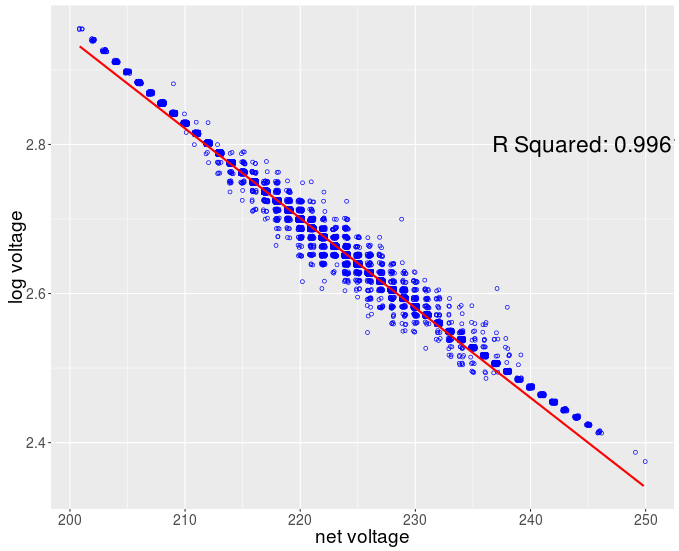
\includegraphics [height = 155pt]{scatter_voltage.png}
\caption{Conversion of Voltage}
\label{fig:Conv_vol}
\end{figure}
%\begin{figure}[here]
%\begin{wrapfigure}{l}{0.3\textwidth}
%  \begin{center}
%  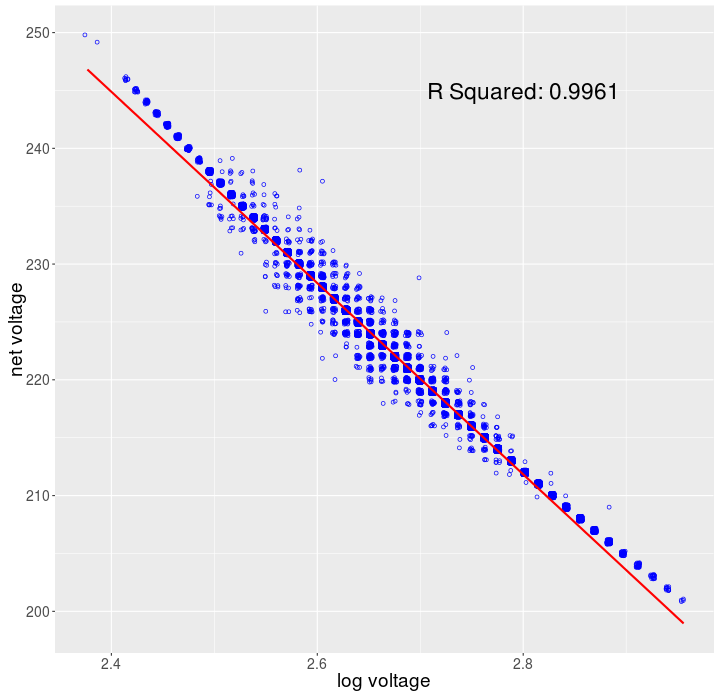
\includegraphics [height = 200pt]{voltage_conversion.png}
%  \caption{Conversion of Voltage}
%  \label{fig:Conv_vol}
%  \end{center}
%\end{wrapfigure}
%\end{figure}
\textbf{Conversion of time}:\\
Another issue about the inconsistency is the time from the log file was all in the downloaded date in Nov, 2004. However, the simple time conversion mentioned in the data collection section fails because of the wrong result\_time in the net dataset. The actual start time of measurments (origin of epoch) should be on 5:10pm, April 27 mentioned in the paper but not April 28. That is demonstrated by a plot of incident PAR of May 1, 2004. I reproduced the similar plots for PAR on May 1st as the original paper, the left plot \ref{fig:wrongTime} used the simple transformation with unreasonable result that radiation was strong in the evening. The right plot \ref{fig:correctTime} with the correct transformation (using 5:10pm, April 27 as epoch 1) shows the reasonable result, and it was consistent to the result in the paper. All time are then transformed to actual time by the epoch information. \\
\textbf{After doing all of these analysis, I found that in the figure 4a in the original paper, the title had showed that epoch 1062 represented 9:35AM on May 1st (thus the epoch 1 should represent 5:10AM on April 27), which corresponded to the correct transformation, so my prior assumption was correct.}\\
\begin{figure}[H]
\centering
\begin{subfigure}{.5\textwidth}
\centering
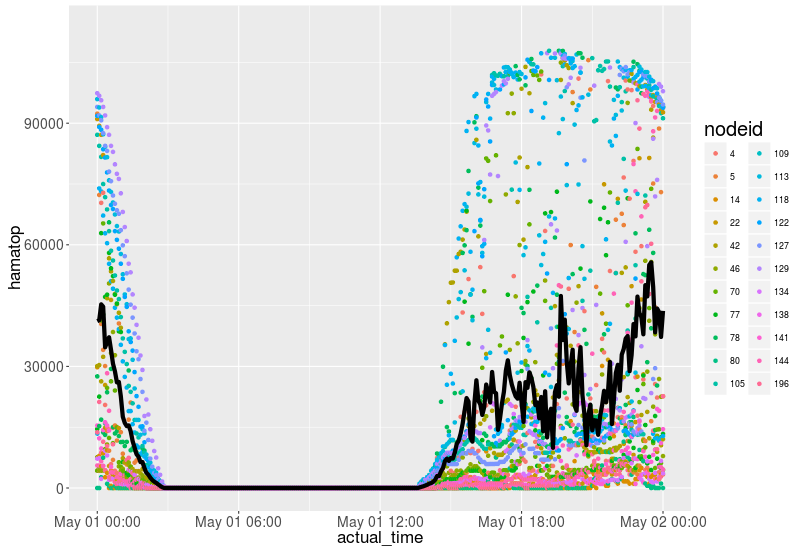
\includegraphics[width=0.95\linewidth]{wrong_time_conversion.png}
\caption{Wrong time conversion PAR}
\label{fig:wrongTime}
\end{subfigure}%
\begin{subfigure}{.5\textwidth}
\centering
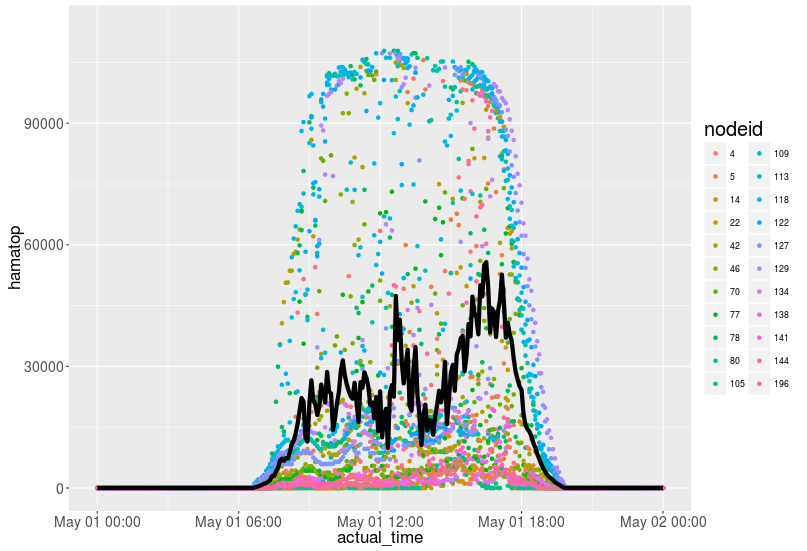
\includegraphics[width=0.95\linewidth]{correct_time_conversion.png}
\caption{Correct time conversion PAR}
\label{fig:correctTime}
\end{subfigure}
\caption{Incident PAR on May 1, 2004, as the similar in the original paper}
\end{figure}%\\
\textbf{Combine of datasets}:\\
Since either of the net dataset or the log dataset had a lot of missing measurements due to the failure of the wireless gateway or the fill-up of the disk space, the first thing was to combine two datasets together to utilize all possible measurements for the interior tree. Notice that there were only three motes still working after June 2nd (correpsonding to epoch 10288), which were 42,127,197, I simply removed the data points after June 2nd to aviod biased plotting. Then I combined the net data and the log data, and removed duplicated entries based on the combination (epoch, nodeid). Notice that because of the issue of voltage, I took the entry from the log data if there was a same entry (same epoch and nodeid) in the net data. If there was no log entry, but a net entry, I would use the voltage transform equation to get a correct voltage for that entry. This raised some minor issues including duplicated data points with the same epoch and nodeid, this often occurred when the result time was just off by less than one second (record multiple times for one point). However, the difference between these duplicated observations was small enough so I just picked up the one that was the first in order. After these, I combined the information in the mote location dataset to the measurement dataset, and there were 3 nodes discarded automatically because of the lack of the information in the mote location dataset (node 65535 (I think it's a numerical error genereated from the computer), node 135, node 100)
\subsubsection{Outlier rejection and detection}
First of all, I removed unreasonable values by common senses and the useless data points pointed out in the paper. To summarize, I removed all missing values with NAs (in the dataset, if one measurement was an NA, then all others were NAs), and removed unreasonable values where the adjusted humidity (RH) was greater than 100 or less than 0 (since RH should be a percentage between 0 and 100). I also discarded the nodes which had distance to the trunk larger than 1 meter, because the original paper pointed out that researchers should mainly focus on the nodes with distance 0.1m to 1m. After this quick operation, the distribution of adjusted humidity did not contain extreme values or outliers.\\
Next, we will focus on the outliers related to low voltage of the sensor, especially for the temperature. The outlier rejection section in the original paper simply deleted all data points with voltage less than 2.4V, which was in fact haste and problematic, because a lot of useful data points that were not outliers were removed. However, checking the voltage information against time for each node would be a good start point to find suspicious nodes that possibly generated outliers. The figure \ref{fig:voltagetime} used the cutoff value 2.4V mentioned in the paper to classify nodes, and it showed that there were 4 nodes (78,134,138,141) that had voltage values less than 2.4V. Then in the right side the figure \ref{fig:strangevoltage} showed the exact temporal trends of voltage. Node 78 and node 138 started from the normal voltage, and gradually decreased to the value lower than 2.4V. Node 134 and node 141 had constant low voltages (they were overlapped in the graph). Yet, after examining the temperatures measured by these node in the figure \ref{fig:fewtemp}, only a part of measurements of node 78 and node 141 showed extreme values (greater than 40 C) in temperature, which should be removed. We observed that node 78 and 141 began to generate outliers after May 7th and May 26th, respectively (the cutoffs are the line dots in \ref{fig:fewtemp}). As for node 134 and node 138, even though they had strange voltage readings, their temperature readings are consistent to other nodes (other nodes are in light blue in the plot), so they should not be discarded as outliers. This also supported my previous conjecture that removing all data points with voltage less than 2.4V in the original paper in fact caused a significant loss of valuable information. This could result from the fact that the voltage readings did not record the actual voltage of the sensor, or the failure of data input. After I removed the extreme values part of the node 78 and 141, the figure \ref{fig:tempnormal} showed that the temporal trends of temperature looked good with no outliers.\\
The cleaned dataset did not show extreme values or outliers in adjusted humidity, incident PAR, and reflected PAR, which indicated that the dataset was ready for the data exploration. The cleaned dataset had 164817 rows.
\begin{figure}[H]
\centering
\begin{subfigure}{.5\textwidth}
\centering
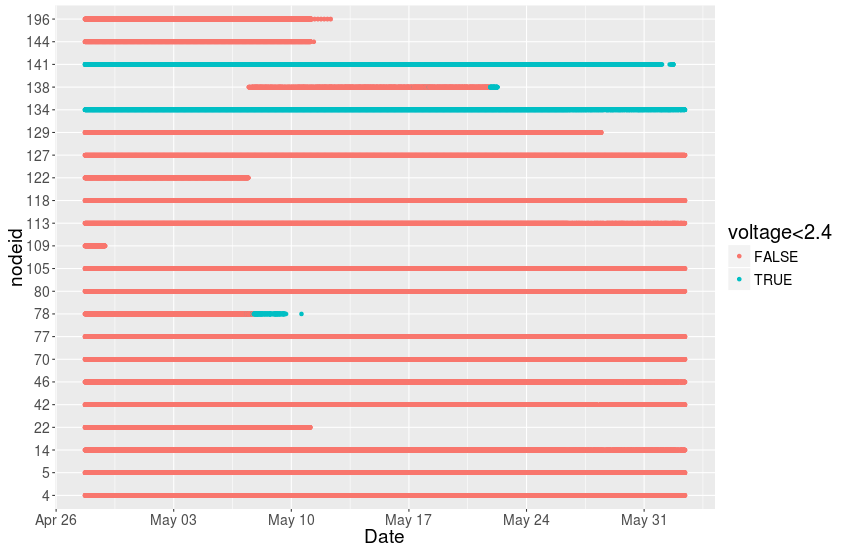
\includegraphics[width=0.88\linewidth]{voltage_time.png}
\caption{Nodes that possibly generated outliers}
\label{fig:voltagetime}
\end{subfigure}%
\begin{subfigure}{.5\textwidth}
\centering
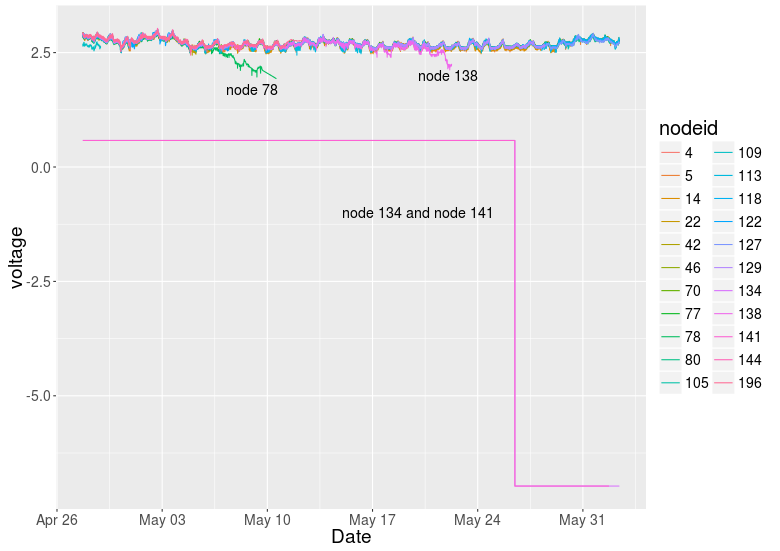
\includegraphics[width=0.88\linewidth]{strange_voltage.png}
\caption{Temporal trends of voltage for nodes}
\label{fig:strangevoltage}
\end{subfigure}
\begin{subfigure}{.5\textwidth}
\centering
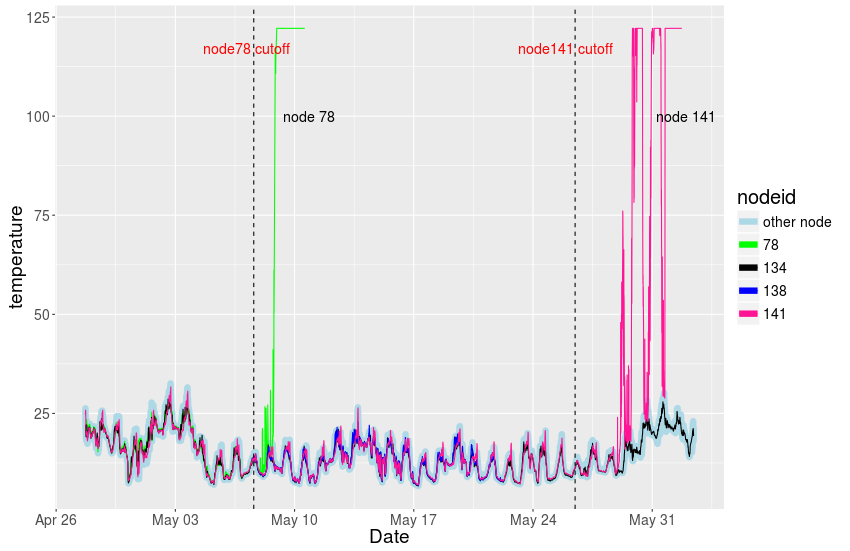
\includegraphics[width=0.88\linewidth]{temp_few.png}
\caption{Temperature of suspicious sensor nodes}
\label{fig:fewtemp}
\end{subfigure}%
\begin{subfigure}{.5\textwidth}
\centering
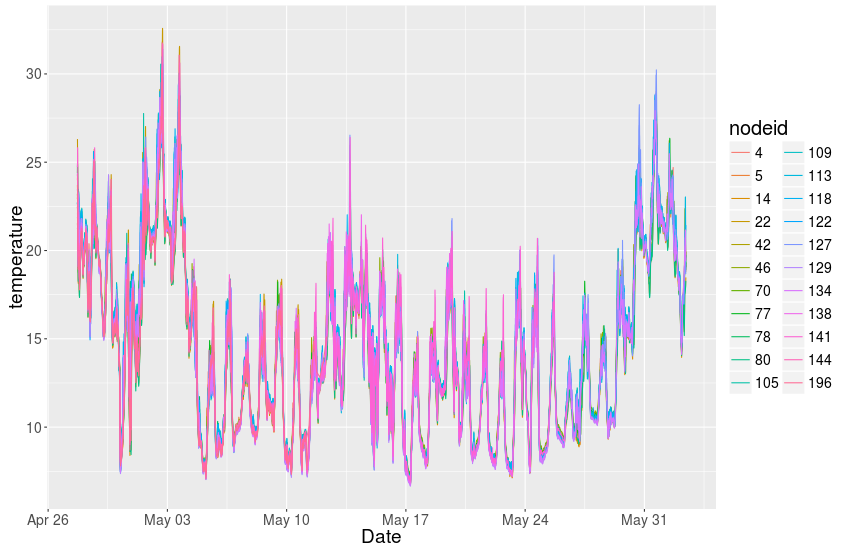
\includegraphics[width=0.88\linewidth]{temp_normal.png}
\caption{Temporal trends of temperature without outliers}
\label{fig:tempnormal}
\end{subfigure}
\caption{Outlier detection for temperature}
\end{figure}%
\subsection{Data Exploration}
The first plot \ref{fig:readingcount} showed the number of valid readings (after data cleaning) against time by a histogram with each bin width=2 days. Notice that since the readings started right on 17:15pm, April 27, therefore the side of the bin did not represent the start of a calendar day. Each bin in the histogram was coloured by sensor nodes with different heights, so one could observe the contribution of readings from each node within a certain period. The plot \ref{fig:heightcount} was a bar plot recording the total number of readings of each node. We should keep in mind that there were nodes like the \textbf{node 109}(64.5m) that only recorded very few readings compared to others, which could cause a bias in the future analysis, since the data from these nodes only presented the climate conditions in the beginning of the research.
\begin{figure}[H]
\centering
\begin{subfigure}{.5\textwidth}
\centering
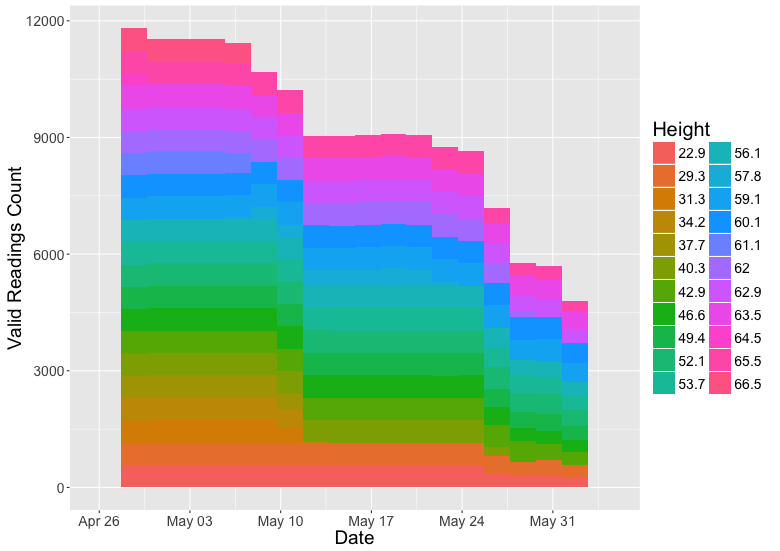
\includegraphics [width=0.9\linewidth,height=0.45\linewidth]{reading_count.png}
\caption{Count of valid readings against time}
\label{fig:readingcount}
\end{subfigure}%
\begin{subfigure}{.5\textwidth}
\centering
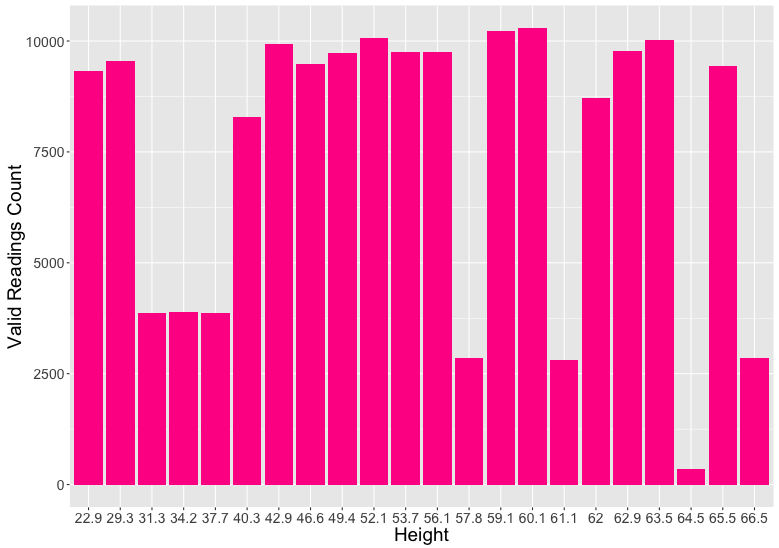
\includegraphics[width=0.9\linewidth,height=0.45\linewidth]{height_count.png}
\caption{Count of valid readings for each sensor}
\label{fig:heightcount}
\end{subfigure}
\caption{Count of valid readings}
\end{figure}%
From \ref{fig:readingcount}, it was clear that the number of readings declined a lot around May 10th and May 26th. Considering the number of readings and to aviod the biasness in height, I would like to choose May 1st data to be a subset, and explore the relationships between hours in a day,height, and climatic measurements. The purpose was similar to the Figure 4 in the original paper, but I scaled the color to show the value of the height variable here to show the '3-D' effects.
\begin{figure}[H]
\centering
\begin{subfigure}{.5\textwidth}
\centering
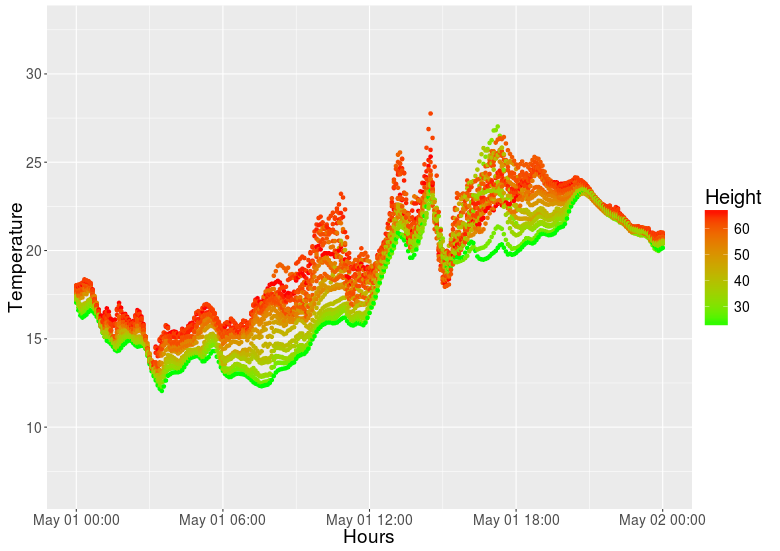
\includegraphics[width=0.88\linewidth,height=0.5\linewidth]{51_temp.png}
\caption{May 1st Temperature against hours}
\label{fig:51temp}
\end{subfigure}%
\begin{subfigure}{.5\textwidth}
\centering
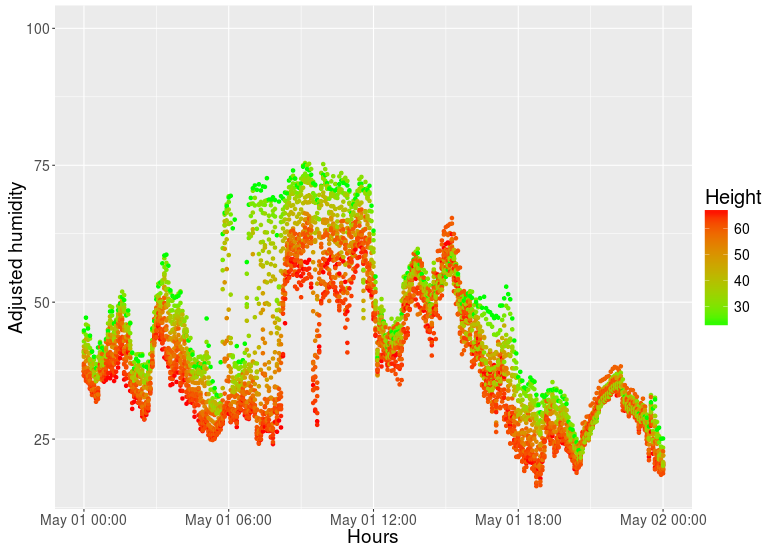
\includegraphics[width=0.88\linewidth,height=0.5\linewidth]{51_humid.png}
\caption{May 1st adjusted humidity against hours}
\label{fig:51humid}
\end{subfigure}
\begin{subfigure}{.5\textwidth}
\centering
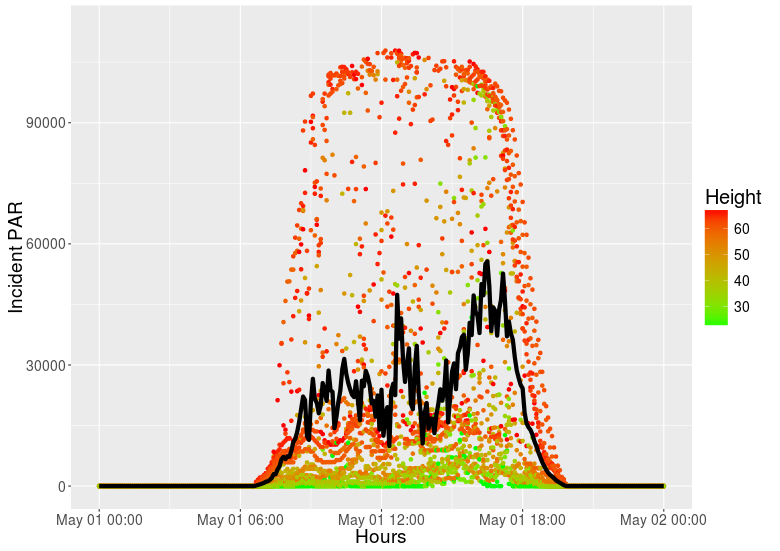
\includegraphics[width=0.88\linewidth,height=0.5\linewidth]{51_par.png}
\caption{May 1st PAR against hours}
\label{fig:51par}
\end{subfigure}%
\begin{subfigure}{.5\textwidth}
\centering
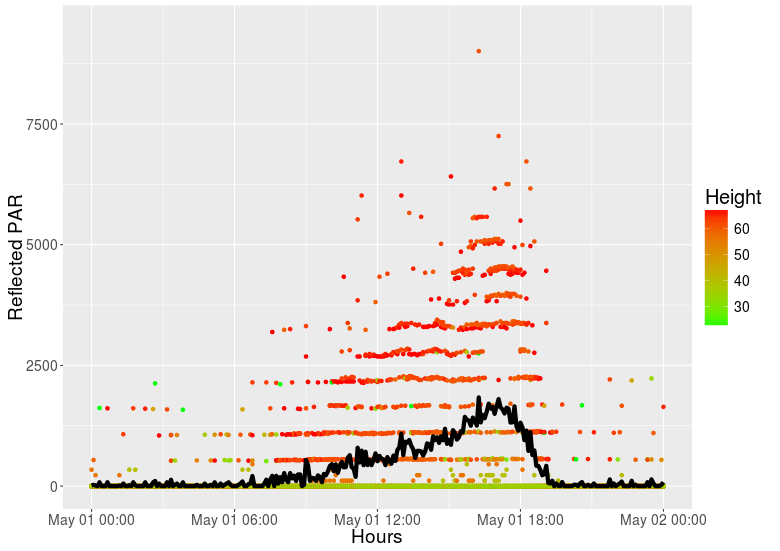
\includegraphics[width=0.88\linewidth,height=0.5\linewidth]{51_rpar.png}
\caption{May 1st reflected PAR against hours}
\label{fig:51rpar}
\end{subfigure}
\caption{May 1st Mesuarements against hours with different heights}
\end{figure}%
The figure \ref{fig:51temp} showed that given a time point on May 1st, height was positively correlated to temperature (red dots sitting upper to the green dots), and the temperature reached its peak on around 2pm. \ref{fig:51humid} showed that the adjusted humidity was negatively associated to height given a certain time on May 1st, where green dots were sitting above. This might suggest a possible negative correlation between humidity and temperature, which would be explored in details next. \ref{fig:51par} showed an apparent hourly cycle of sun radiation matches the comon sense, and higher nodes in red generally had larger incident PAR values. The line in black was the average of incident PAR against time, it reached peak at around 1pm and 5pm. In \ref{fig:51RPAR}, the reflected PAR showed the similar relationship versus the height, however it reached the peak at around 5pm. Considering both \ref{fig:51temp} and \ref{fig:51par}, we see that as the PAR started to spike from zero at around 6am, the temperature began to increase. As the radiation decreased, the temperature fall.\\
I will examine the above exploration results on the whole dataset in the finding section to see if those relationships are still hold.\\
\begin{figure}[H]
\centering
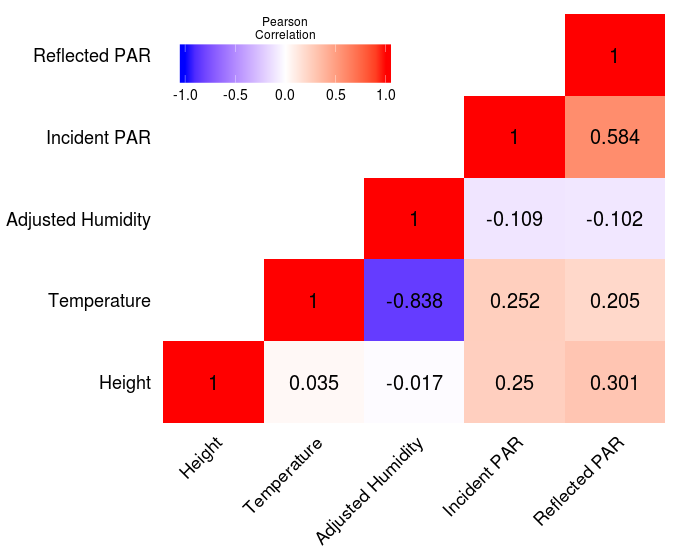
\includegraphics [height = 170pt]{cor_mat.png}
\caption{Correlation heatmap of measurements}
\label{fig:cormat}
\end{figure}
\begin{figure}[H]
\centering
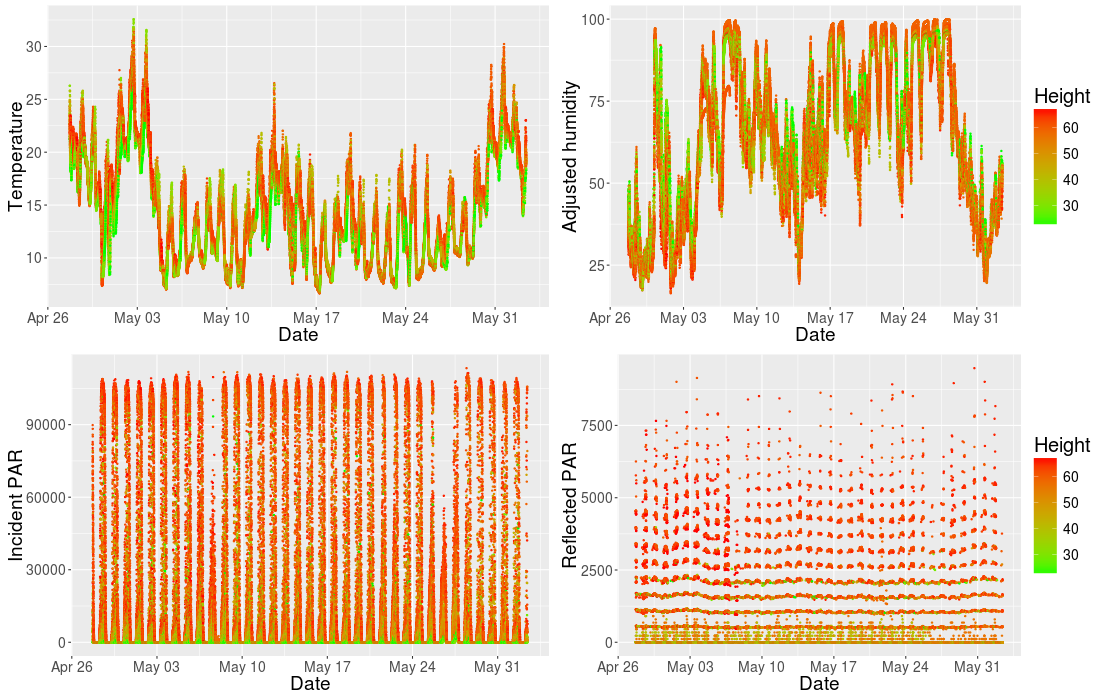
\includegraphics [width=0.95\linewidth,height=0.55\linewidth]{daily_cycle.png}
\caption{Daily cycle of measurements}
\label{fig:dailycycle}
\end{figure}
Next I will focus on the relationship among measurements and spatial data, since all four measurements: temperature, adjusted humidity, incidient PAR and reflected PAR were continuous values, and the spatial measurment height was also a countinuous value, it was reasonable to start with a correlation matrix. The figure \ref{fig:cormat} showed that there was a strong negative correlation (-0.838) between adjusted humidity and temperature (marked in blue). Besides, the incident PAR and the reflected PAR had moderate positive correlation. I will further explore the relationships between humidity and temperature in the findings section.\\
After exploring the hourly pattern of measurements within one day, I would like to check the daily cycles of climatic measurements to see if those measurements were significantly different during April 27 to June 2. From \ref{fig:dailycycle}, we can see that the temperature was not stationary through the research period. The average temperatures in the beginning and the end of the May were signifcantly higher than average temperatures in mid-May. We should keep this in mind that perhaps it would be hard to generalize the result because of the significant climatic change through time, and the May 1st data in the previous part of the exploration might not be representative. Moreover, the shape of the time series of humidity was approximately the inverse of the temeperature, which possibly indicated a negative correlation. Besides, we can still observe that there was a strong seasonal pattern for the incident PAR and the reflected PAR, which also followed the common sense of sunlight behaviors. Unlike temperature and humidity, the radiation variables incident PAR and reflected PAR behaved similarly day by day, except for May 7th and May 27th, where PAR and RPAR were significantly lower, which could result from the rain or cloud.\\
Finally in the last part of the data exploration section, I will briefly see how direction of nodes affect the sunlight radiation (incident PAR). Notice that since the data cleaning process has discarded all data points with distance larger than 1 meter, so the most nodes in the cleaned dataset were in the direction of south west, thus it was an imbalanced classification to classify data points using directions. Here I just used the data from 6:00AM to 8:00PM in each day, because it would be pointless to analyze the sunlight radiation in night. The figure \ref{fig:boxpar} shows that the overall distribution of incident PAR was higher for the direction Southwest and West Southwest. However as I plotted the Height against Direction in the right side, we found that nodes with direction SW and WSW had higer spatial positions, which might bring more sunlight radiation, and thus the variation was probably not contributed from the different directions.
\begin{figure}[H]
\centering
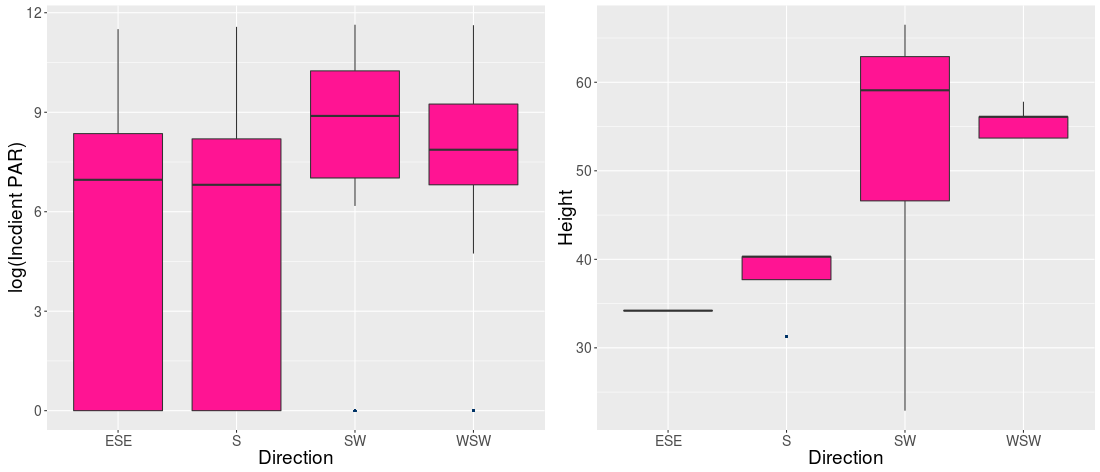
\includegraphics [width=0.95\linewidth,height=0.3\linewidth]{box_par.png}
\caption{Boxplot of Direction and sunlight radiation in day time}
\label{fig:boxpar}
\end{figure}
\section{Graphical Critique}
\paragraph{3a}
The figure 3a in the original paper examines the univariate distributions of four measurements: humidity, temperature, incident PAR, and reflected PAR by four histograms. Overall the graphs present the distributions clearly. However, the graph for the temperature uses too wide interval on the x-axis, and this results in the conclusion that temperature has unimodal distributions while they could have multiple modes near 10 instead. One quick imporvement is to narrow the interval, and an alternative could be a density plot with detailed information instead of the histogram. Besides, for PAR and RPAR, it would be more relevant to use the daily data, because the sunlight radiation will definitly be zero during night time.
\paragraph{3b}
The figure 3b tries to show how do the distributions for measurements vary in time. In each graph, there is one box-plot for the distribution in one day. The first two plots basically convey the information, and give readers a sense of the change of medians over time. However the last two plots fail to convey useful information, since the distributions are highly skewed and the boxes are tiny. A quick improvement is to remove the night values for incident and reflected PARs, otherwise all daily values are certainly outliers while they are valuable. Another issue to mention is the date range, after June 2 there were only 3 working sensors, thus that was why the distributions after June 2 were narrower than previous days, the author should point it out explicitly. Besides, an alternative to these plots could be representing the density of data points by using different scale of colors instead of box plots. 
\paragraph{3c}
The figure 3c is an analog to the figure 3b, where it represents the distributions of measurements against time by horizontal box-plots. The plot is not persuasive because the confounding effects of time, but the problem has been solved in 3d. One thing to mention is that the author plotted height as a categorical variable in the y-axis distant equally, and it is better to clarify to avoid the misunderstanding that the y-value is directly proportional to the numerical values of height.
\paragraph{3d}
The figure 3d eliminates the time effect by differencing the measurements from their means for each node, and plot them against height. The plots are actually informative than 3c, however it is not as straightforward as other graphs, the caption should be more clear.\\
Overall the title and axis texts are too small to read in figure 3 considering there is still quite a lot white space horizontally 
\paragraph{Figure 4}
The left plots in figure 4 show the change of temperature, humidity, incident PAR, reflected PAR against time on May 1st, 2004. Each line represents the different sensor motes in different colors in the first two plots. Additionally, there is a vertical line marking the dramatic change of slopes. The plot should include a legend specifying that different colors are denoting different nodes, otherwise if no legend is used then the plot should just use one color instead. In the plots for PAR and reflected PAR, the report does not assign different colors based on different sensors, which is inconsistent to the first two plots. On the right hand side, the scatter plots show the relationship between four measurements and the height variable. There are two different colors of scatters, which should be specified in the lengend aside from the scatter plot. Generally, the figure try to convey the relationships between measurements, time, and height. Therefore, plotting in 3D could be a better alternative. An alternative of the figure 4 has been shown in the data exploration section, where I use the color to show the effects of height in stead of using another plot.
\section{Findings}
\subsection{First finding: Hourly trends of sunlight radiation}
In the data exploration section, I have explored the hourly trend of incident PAR and reflected on May 1st, 2004. However, it would be more persuasive if I used the data points from all dates to show the hourly pattern.\\
In the analysis, the incident PAR and reflected PAR were averaged over each node's life (unit is a day). For instance, node 5 would have only one incident PAR value for 19:05pm, and the value was computed by averaging 44 days. \ref{fig:parrparheat} and \ref{fig:parrparpoint} show that \textbf{by averaging over the aggregate dataset, both the incident PAR and the reflected PAR had strong hourly pattern that started to increase from zero at around 6AM every day, and began to decline toward zero from 4:30PM until 8PM. Generally, higher sensors received more sunlight radiation (direct PAR and reflected PAR) during day time than lower sensors, and lower sensors had less sunlight radiation because of the obscureness of canopy and leaves.}\\ Notice that the color uses for PAR and height gradient are consistent to the data exploration and the third finding.
Cross-validating the accuracy of the plot by checking the database of California sunrise time for Sonoma county \cite{sunrise}, the time of sunrise had a range 6:18AM to 5:48AM from April 27 to June 2, and the time of sunset had a range of 7:57PM to 8:28PM. These results were consistent to the my first finding. Moreover, since almost all sensors were placed to the west direction (either SW or WSW), thus it would be reasonable that the peaks of incident PAR and reflected PAR were in the afternoon (around 4:30 pm). 
\begin{figure}[H]
\centering
\begin{subfigure}{.5\textwidth}
\centering
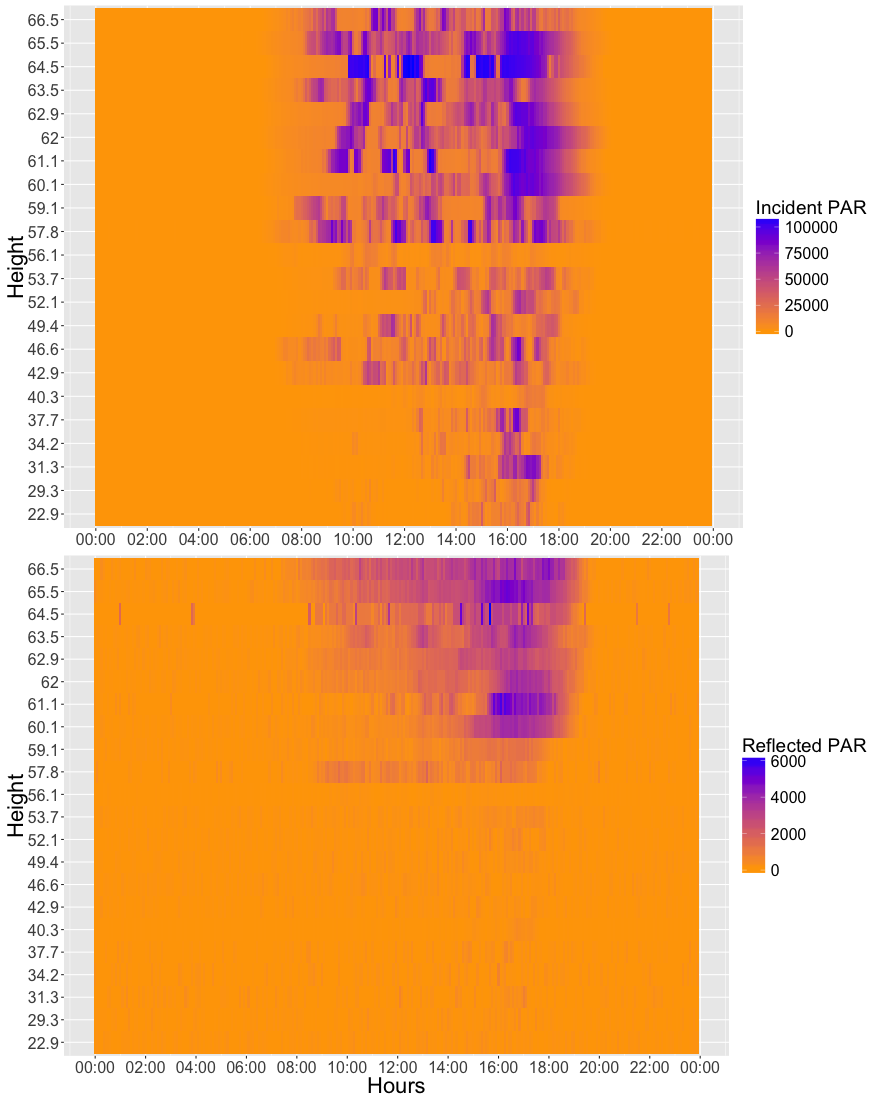
\includegraphics [width=1\linewidth,height=1.1\linewidth]{find11.png}
\caption{Heat map for radiation with spatial gradient}
\label{fig:parrparheat}
\end{subfigure}%
\begin{subfigure}{.5\textwidth}
\centering
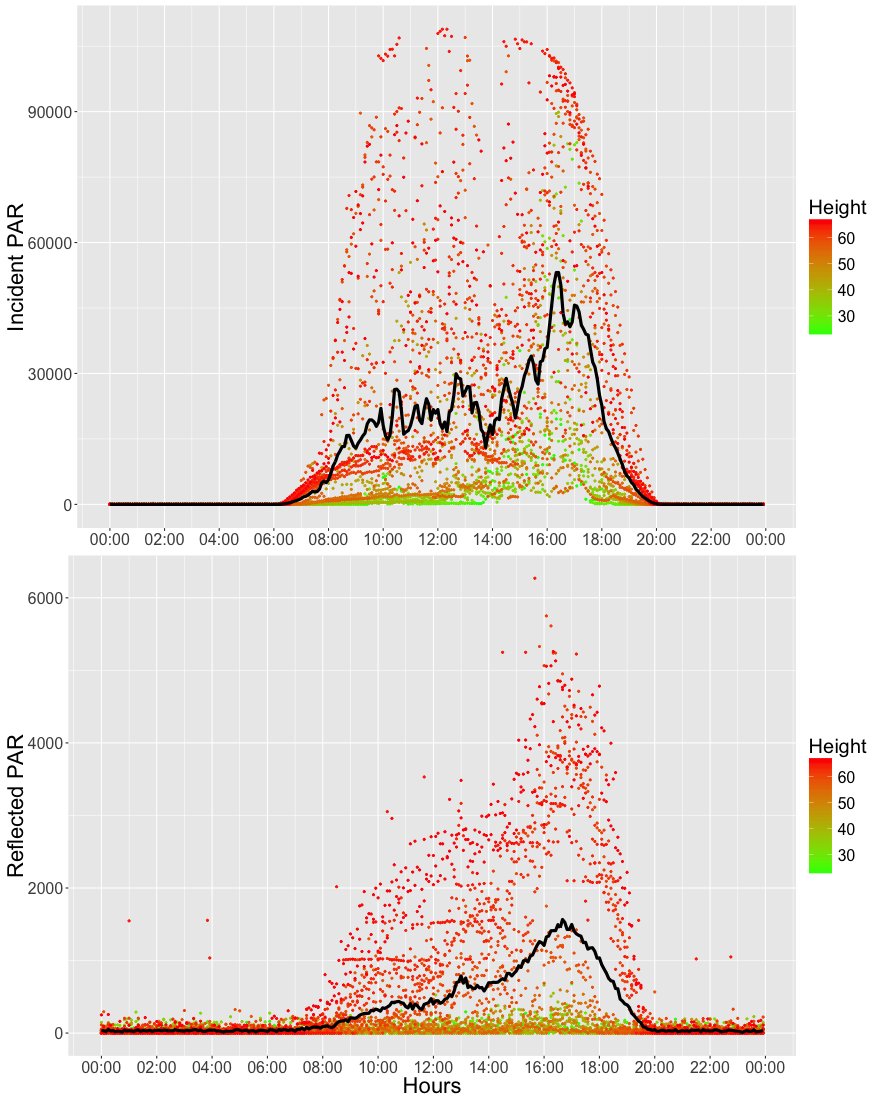
\includegraphics[width=1\linewidth,height=1.1\linewidth]{find12.png}
\caption{Hourly trend for sunlight radiation}
\label{fig:parrparpoint}
\end{subfigure}
\caption{Hourly trend for sunlight radiation with spatial gradient}
\end{figure}

\subsection{Second finding: Temporal trends of temperature and humidity}
\begin{figure}[H]
\centering
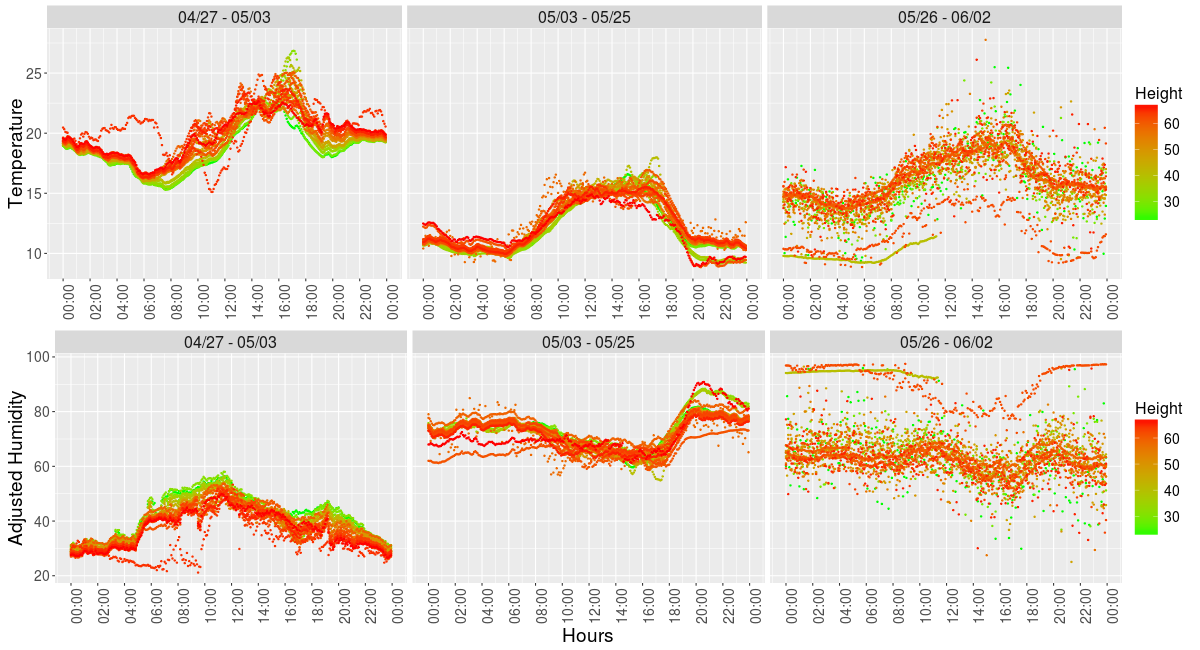
\includegraphics [width=0.95\linewidth,height=0.5\linewidth]{find_2.png}
\caption{Hourly trends of humidity and temperature}
\label{fig:find2}
\end{figure}
The second finding is about the hourly trend of temperature and humidity in 3 different time periods. As it's shown on the data exploration section \ref{fig:dailycycle}, the temperature (humidity) was particularly high (low) around May 1st and May 30th. Since temperature and humidity had a lot of variation among dates, it was hard to generalize one hourly pattern by averaging over the entire dataset like the Finding 1. In appendix, I have added the aggregate graph \ref{fig:app1} to show that it was difficult to see the pattern. Therefore I divided the research period into 3 time intervals: 4/27-5/3 (begin), 5/4-5/25 (middle), 5/26-6/26, and averaged temperature over these three intervals to get 3 different hourly trends for temperature and adjusted humidity.\\
From \ref{fig:find2}, I found that \textbf{despite the fact that these 3 periods had different mean levels of humidity and temperature, the changing patterns were similar. In average, the temperature (adjusted humidity) started to increase (decrease) in the morning around 7AM, and reached the maximum(minimum) in the afternoon around 3PM, then gradually decreased (increased) until evening.} The only exception was the adjusted humidity from April 27 to May 3, where the daytime humidity was higher than the night time humidity, and the pattern was nearly the reverse of the pattern from 5/3 to 6/2. As we color coded the data points by heights, height did not seem to be a strong spatial confounding factor to temperature and humidity except for the period 4/27 to 5/3, where height positively correlated to temperature and negatively correlated to humidity.\\
To make some clarifications, one should notice that there were less sensor nodes working in the period 5/26 to 6/2, thus the mean dots in that period were not as stable as before.
\subsection{Third finding}
\begin{figure}[H]
\centering
\begin{subfigure}{1\textwidth}
\centering
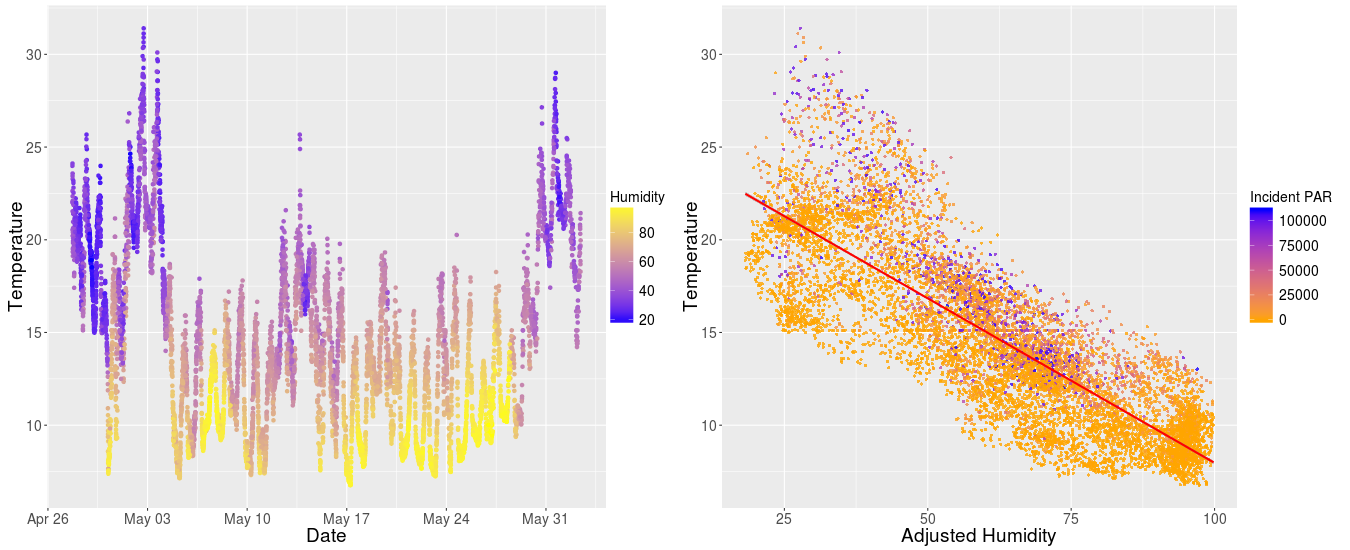
\includegraphics [width=0.9\linewidth,height=0.33\linewidth]{random_corr.png}
\caption{Temperature versus Humidity: randomly sampled 10000 data points}
\label{fig:randomcorr}
\end{subfigure}
\begin{subfigure}{1\textwidth}
\centering
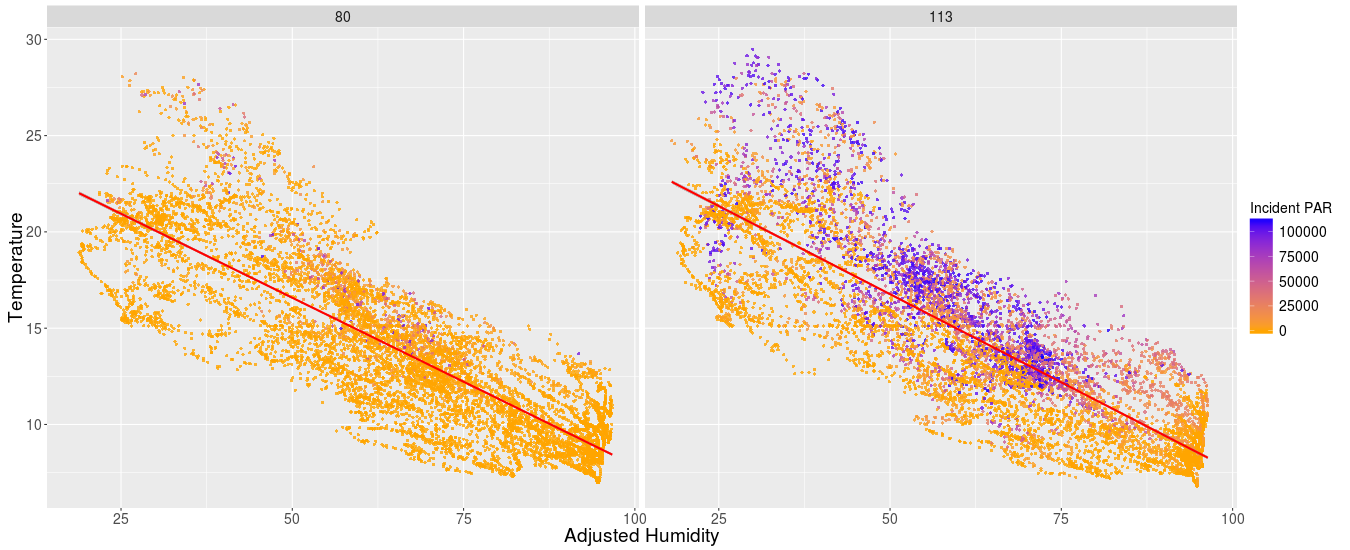
\includegraphics[width=0.9\linewidth,height=0.35\linewidth]{temp_humid_scatter2.png}
\caption{Temperature versus Humidity in dfferent Heights: Node 80 (low) and 113 (high)}
\label{fig:scatter2}
\end{subfigure}
\caption{Negative Association between temperature and humidity}
\end{figure}
My third finding was that \textbf{humidity (the adjusted humidity) was negatively correlated to temperature for sensor motes in dfferent heights. For higher motes, low humidity together with high PAR usually indicated even higher temperature than just explaining the variation of temperature by humidity.} In the data exploration, from \ref{fig:cormat} and \ref{fig:dailycycle}, I had the conjecture that temperature was negatively associated with humidity. Since plotting hundreds of scatter points would cause a serious over-plotting problem, I first randomly sampled 10000 data points to show the general correlation. In \ref{fig:randomcorr}, the left plot presented the sampled temperature against date with color scaled by humidity. While temperature was low, the points were more likely to be yellow, indicating a high humidity. The right graph was a standard scatter plot with the regression line, and the color was coded by incident PAR.\\
Except for the negative correlation, we also found that high PAR value points in deep blue often sit above the regression line. To search for an in-depth explanation about this phenomena, I plot the scatter plots for node 80 (22.9m) and node 113 (65.5m) \ref{fig:scatter2}, because the height of the node was highly correlated to PAR by the first finding. In the higher node (65.5m), most of the high PAR value points were sitting above the regression line, indicating that they were "under estimated" in temperature. \textbf{For higher nodes, incident PAR explained some extra variation (extra sum of error squares) that were not catched by humidity.} Future research could focus on the interaction between Height and PAR, and possible come up with a better model.
\section{Discussion}
For future analysis on the redwood dataset, I would concentrate more on other aspects that were not discussed in this paper. Due to the restriction in page limits and time, I have narrowed my focus on the interior tree with sensor nodes near the trunk (Distance less than 1m) in the data cleaning process. With that being said, I was not able to do the comparison between the interior tree and the edge tree, which might be meaningful for future research. Besides, the majority effort was spend on the data cleaning and outlier rejection. Nevertheless, data cleaning finalized the dataset that were actually analyzed, so it determined the scope of the study in some degrees. The failure in data cleaning could cause fatal problems.\\
The other limitation of this study was the lack of advanced models related to physical laws and statistical methods. For instance, I would like to check the interaction terms between mesurements and spatial values to see if a more comprehensive model will emerge. \\
Overall, the size of the dataset was not the main restriction for today's computers, even though that could be a problem back in 2005 when the original paper was published. The biggest difficulty was about the lack of clarification of variables. For instance, there were no text describing variables like parent, depth, and the original paper did not talk about the edge tree's background, which made the comparison difficult. Besides, a lot of dirty data problems and mistakes were not apparent at the first look, exhaustive exploration were needed to detect them.

\section{Conclusion}
In this report, I first briefly introduced and cleaned the dataset. Next I have explored the dataset searching for possible meaningful findings, and some interesting exploring results were recorded in graphics in this section. Finally I presensted three meanignful findings regarding the temporal trends of climatic measurements and correlation analysis. Unlike the original paper in 2005 \cite{tolle2005macroscope} spending a lot on explaining the methodology, the report focused on exploratory data analysis of multi-dimensional climatic measurements by data visualization.

\section{Appendices}
\subsection{Appendix for Finding 2}
\begin{figure}[H]
\centering
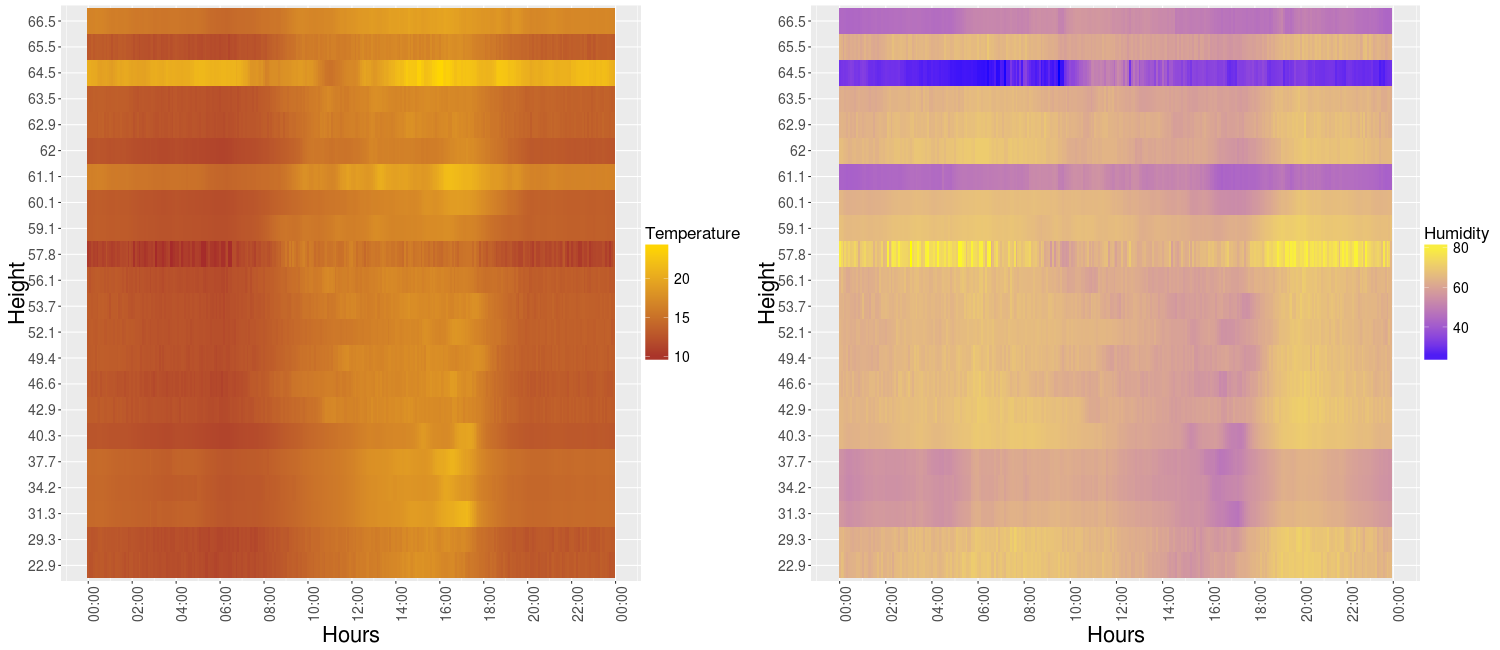
\includegraphics [width=1\linewidth,height=0.35\linewidth]{app_1.png}
\caption{Heatmap of humidity and temperature on the aggregating dataset}
\label{fig:app1}
\end{figure}
Please refer to the section second finding to see the instructions of these plots.
% the `Acknowledgments` section is required if you discussed the project
% with anyone else.
\section*{Acknowledgments}
I have consulted with Siyao Chang, Cenzhuo Yao, and Mengfei Jiang for this project. Specifically for the data cleaning part, the purpose, and the scope of the study, I appreciate their discussion and help. 

\bibliographystyle{plain}
\bibliography{sensor}

\end{document}
